\documentclass[tikz,border=2pt]{standalone}
\usepackage{amsmath,amssymb}
\usetikzlibrary{arrows.meta}
\begin{document}
% (s,S) = (2,8) policy, demands 2,3,1,4,0,3,2,5,1,2 in periods 1..10, P_1 = 8.
% Each period shows the start position P_k (left half) and the end position P_k' (right half).
% When P_k' <= s = 2 (end of periods 3, 6 and 8) the order S - P_k' lifts the position back to S = 8:
% orders 6, 7, 7 at the starts of periods 4, 7, 9; otherwise no order.
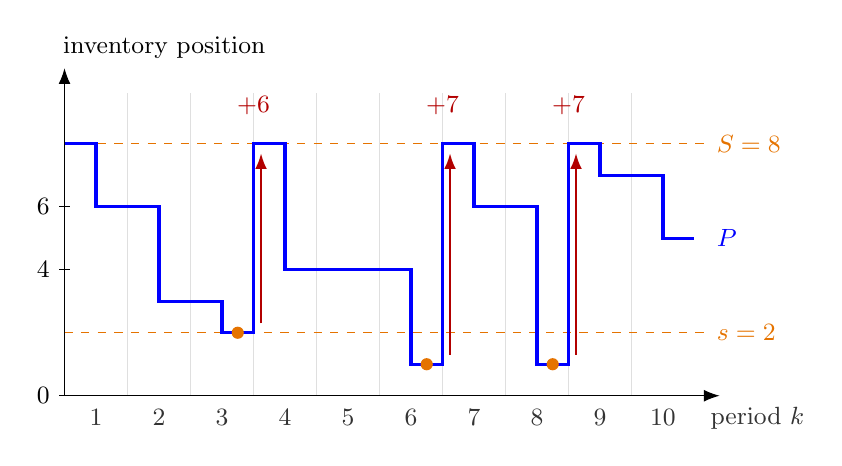
\begin{tikzpicture}[font=\small, >={Latex[length=2mm]}, x=0.8cm, y=0.4cm]
  \foreach \k in {1,...,9} {\draw[gray!25] (\k,0) -- (\k,9.6);}
  \draw[->] (0,0) -- (10.4,0);
  \draw[->] (0,0) -- (0,10.4) node[anchor=south west, xshift=-4pt] {inventory position};
  \foreach \v in {0,4,6} {\draw (0.08,\v) -- (-0.08,\v) node[left] {$\v$};}
  \foreach \k in {1,...,10} {\node[gray!40!black] at (\k-0.5,-0.7) {$\k$};}
  \node[gray!40!black, anchor=west] at (10.1,-0.7) {period $k$};
  % policy levels
  \draw[orange!90!black, thin, dashed] (0,8) -- (10.2,8) node[right] {$S=8$};
  \draw[orange!90!black, thin, dashed] (0,2) -- (10.2,2) node[right] {$s=2$};
  % position path
  \draw[blue, very thick] (0,8) -- (0.5,8) -- (0.5,6) -- (1,6) -- (1.5,6) -- (1.5,3) -- (2,3) -- (2.5,3) -- (2.5,2) -- (3,2) -- (3,8) -- (3.5,8) -- (3.5,4) -- (4,4) -- (4.5,4) -- (5,4) -- (5.5,4) -- (5.5,1) -- (6,1) -- (6,8) -- (6.5,8) -- (6.5,6) -- (7,6) -- (7.5,6) -- (7.5,1) -- (8,1) -- (8,8) -- (8.5,8) -- (8.5,7) -- (9,7) -- (9.5,7) -- (9.5,5) -- (10,5);
  \node[blue, anchor=west] at (10.2,5) {$P$};
  % end-of-period positions at or below s trigger an order
  \foreach \x/\y in {3/2,6/1,8/1} {\fill[orange!90!black] (\x-0.25,\y) circle (2.2pt);}
  % orders
  \foreach \x/\q in {3/6,6/7,8/7} {\node[red!70!black, anchor=south] at (\x,8.6) {$+\q$};}
  \foreach \x/\y in {3/2,6/1,8/1} {\draw[red!70!black, ->, thick] (\x+0.12,\y+0.3) -- (\x+0.12,7.7);}
\end{tikzpicture}
\end{document}
